\section{Implementación}
\label{sec:impl}

\subsection{Placa y componentes}
La Fig.~\ref{fig:placa} muestra la placa ensayada y la Tabla~\ref{tab:bom}, los componentes del circuito de la Fig.~\ref{fig:circuito}, con el tipo elegido para cada uno según la Sección~\ref{sec:diseno}.

\begin{figure*}[!t]
\centering
\begin{subfigure}[b]{0.42\textwidth}
\centering
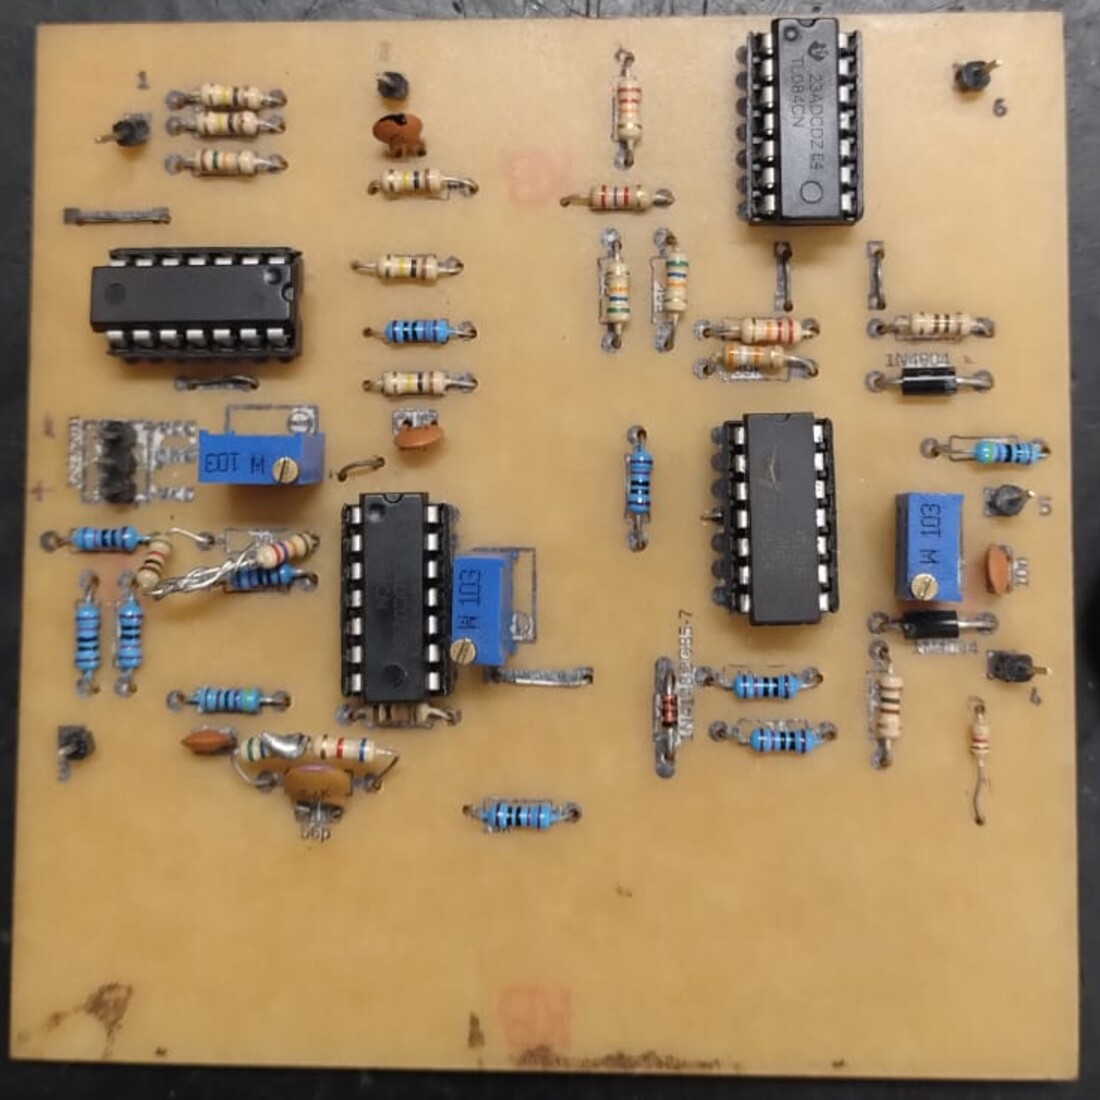
\includegraphics[width=\linewidth]{figuras/placa_superior.jpg}
\caption{Lado de componentes.}
\end{subfigure}\hspace{0.04\textwidth}%
\begin{subfigure}[b]{0.42\textwidth}
\centering
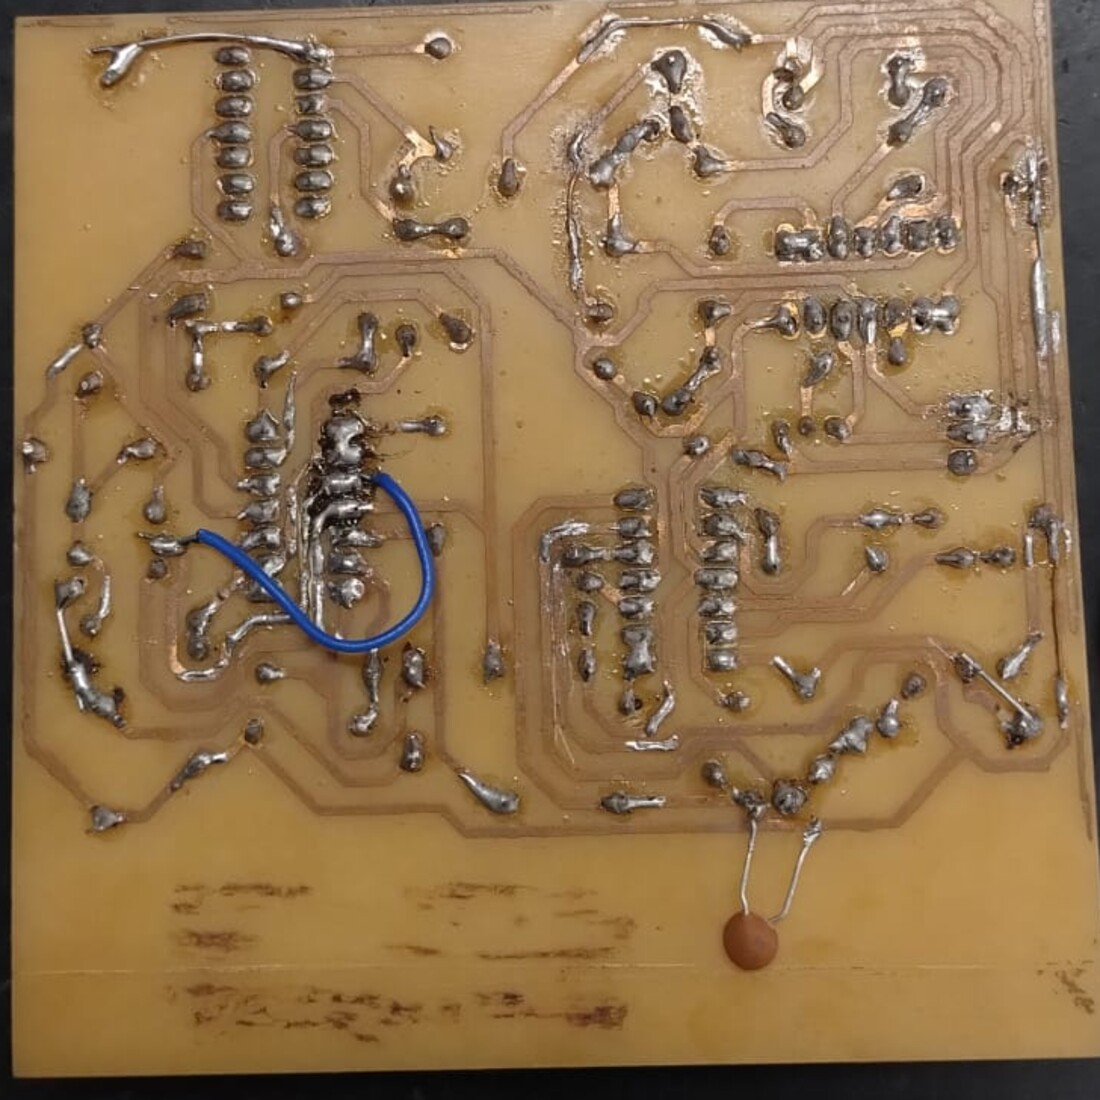
\includegraphics[width=\linewidth]{figuras/placa_inferior.jpg}
\caption{Lado de pistas.}
\end{subfigure}
\caption{Placa ensayada.}
\label{fig:placa}
\end{figure*}

\begin{table}[!htb]
\centering
\caption{Lista de componentes.}
\label{tab:bom}
\footnotesize
\setlength{\tabcolsep}{3pt}
\begin{tabular}{@{}>{\raggedright}p{2.5cm}l>{\raggedright\arraybackslash}p{3.2cm}@{}}
\toprule
\textbf{Referencia} & \textbf{Valor} & \textbf{Tipo} \\
\midrule
U1, U2, U3 & TL084CN & DIP-14 \\
$R_1$, $R_9$ & \SI{15}{\kilo\ohm} & Película metálica, \SI{1}{\percent} \\
$R_2$ a $R_8$, $R_{10}$ a $R_{13}$, $R_{15}$, $R_{F8}$ & \SI{10}{\kilo\ohm} & Película metálica, \SI{1}{\percent} \\
$R_{14}$ & \SI{20}{\kilo\ohm} & Película metálica, \SI{1}{\percent} \\
$R_I$ & \SI{5,6}{\kilo\ohm} & Película metálica, \SI{1}{\percent} \\
$R_F$ & \SI{1}{\mega\ohm} & Película metálica, \SI{1}{\percent} \\
$R_D$ & \SI{31,6}{\kilo\ohm} & Película metálica, \SI{1}{\percent} (E96) \\
$R_S$ & \SI{1}{\kilo\ohm} & Película metálica, \SI{1}{\percent} \\
$R_{S4}$, $R_{F4}$ & \SI{4,7}{\kilo\ohm} & Película metálica, \SI{1}{\percent} \\
$R_Z$ & \SI{470}{\ohm} & Película metálica, \SI{0,25}{\watt} \\
$P_1$, $P_2$, $P_3$ & \SI{10}{\kilo\ohm} & Preset multivuelta \\
$C_1$ & \SI{4,7}{\nano\farad} & Poliéster, \SI{5}{\percent} \\
$C_D$, $C_4$ & \SI{1}{\nano\farad} & Poliéster, \SI{5}{\percent} \\
$C_F$ & \SI{56}{\pico\farad} & Cerámico NP0 \\
$C_C$ & \SI{1}{\micro\farad} & Poliéster \\
Desacople (por integrado) & \SI{100}{\nano\farad} + \SI{10}{\micro\farad} & Cerámico + electrolítico \\
$D_{Z1}$ & 1N750 & Zener \SI{4,7}{\volt}, \SI{500}{\milli\watt} \\
$D_1$, $D_2$ & 1N4004 & Rectificador \SI{1}{\ampere} \\
\bottomrule
\end{tabular}
\end{table}

\subsection{Procedimiento de ajuste}
\label{sec:ajuste}
Los tres presets se ajustan en el orden en que afectan a las señales, porque cada uno cambia todo lo que está después:
\begin{enumerate}[leftmargin=*, nosep]
    \item Sin señal de entrada, verificar las tensiones de alimentación y la del zener.
    \item Con un multímetro en la salida de U1B, llevar $\Vrefd$ a \SI{1,25}{\volt} con $P_1$; con el multímetro en la salida de U2D, llevar $\Vrefu$ a \SI{1}{\volt} con $P_2$.
    \item Conectar el generador (cuadrada de \SI{0}{} a \SI{2,5}{\volt}, \SI{4,3}{\kilo\hertz}) y esperar un segundo, para que se cargue $C_C$.
    \item Con el osciloscopio en continua, verificar que la señal 1 vaya de \SI{-1}{} a \SI{1,5}{\volt}; si no, retocar $P_2$. Medir el valor medio de la señal 2 con el multímetro y, si no es \SI{1,25}{\volt}, retocar $P_1$: así se compensan también los \emph{offsets} de los operacionales.
    \item Ajustar $P_3$ para que los impulsos de la señal 4 tengan \SI{1}{\volt} de pico.
\end{enumerate}

\subsection{Medición}
La placa se alimentó con la fuente partida del laboratorio y se excitó con el generador de funciones ajustado a una cuadrada de \SI{0}{} a \SI{2,5}{\volt} y \SI{4,3}{\kilo\hertz}. Las señales se registraron con un osciloscopio digital Rigol, en continua; la Fig.~\ref{fig:capturas} reúne las seis capturas.

Para compararlas con la simulación se digitalizaron. Cada captura tiene una retícula de 12 por 8 divisiones de 25 píxeles, así que cada píxel equivale a $1/25$ de división en tensión y en tiempo, y la traza amarilla se convierte en una tabla tensión--tiempo. Con las bases de tiempo usadas, un píxel equivale a \SI{2}{\micro\second} en las capturas 1 a 3 y a \SI{4}{\micro\second} en las capturas 4 a 6, de modo que los detalles más breves que eso no se resuelven.

\begin{figure*}[!t]
\centering
\begin{subfigure}[b]{0.32\textwidth}
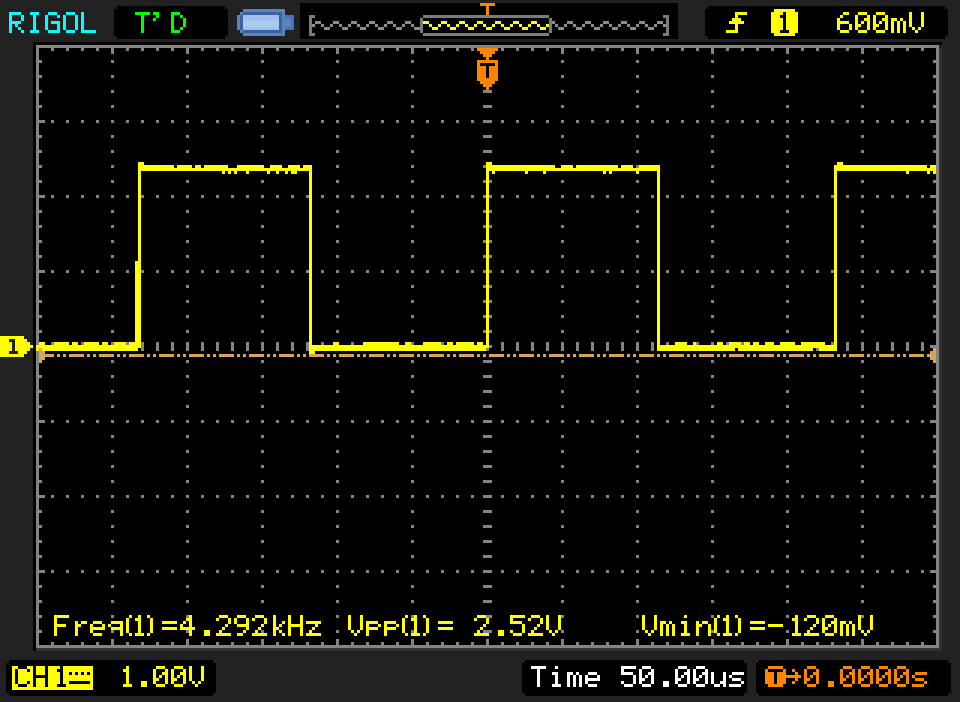
\includegraphics[width=\linewidth]{figuras/osc_1.png}
\caption{Entrada (\SI{1}{\volt\per div}, \SI{50}{\micro\second\per div}).}
\end{subfigure}\hfill
\begin{subfigure}[b]{0.32\textwidth}
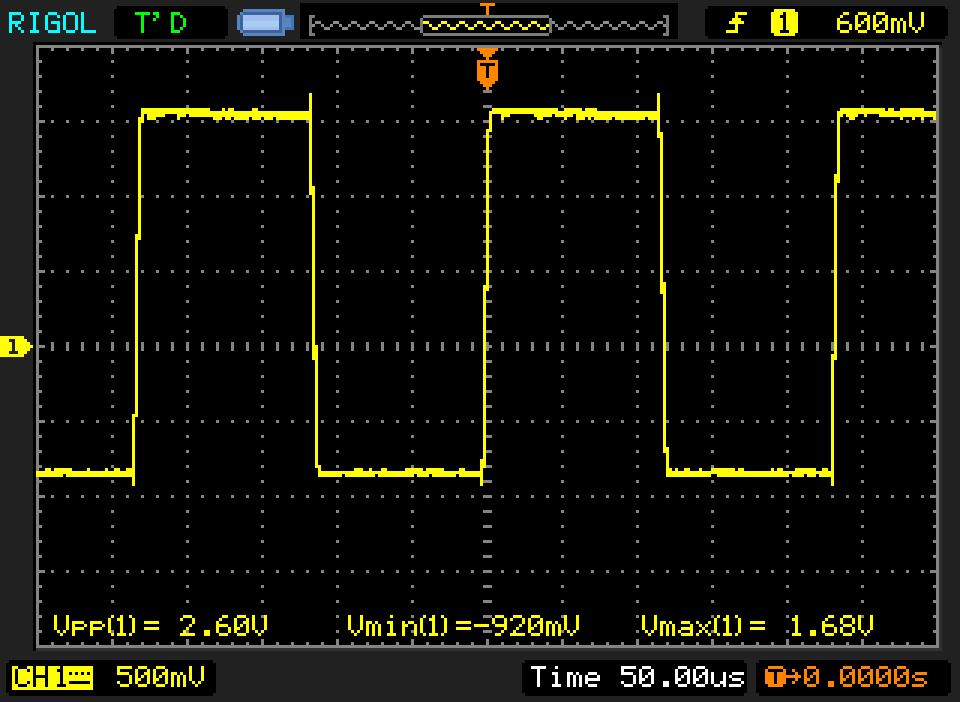
\includegraphics[width=\linewidth]{figuras/osc_2.png}
\caption{Señal 1 (\SI{0,5}{\volt\per div}, \SI{50}{\micro\second\per div}).}
\end{subfigure}\hfill
\begin{subfigure}[b]{0.32\textwidth}
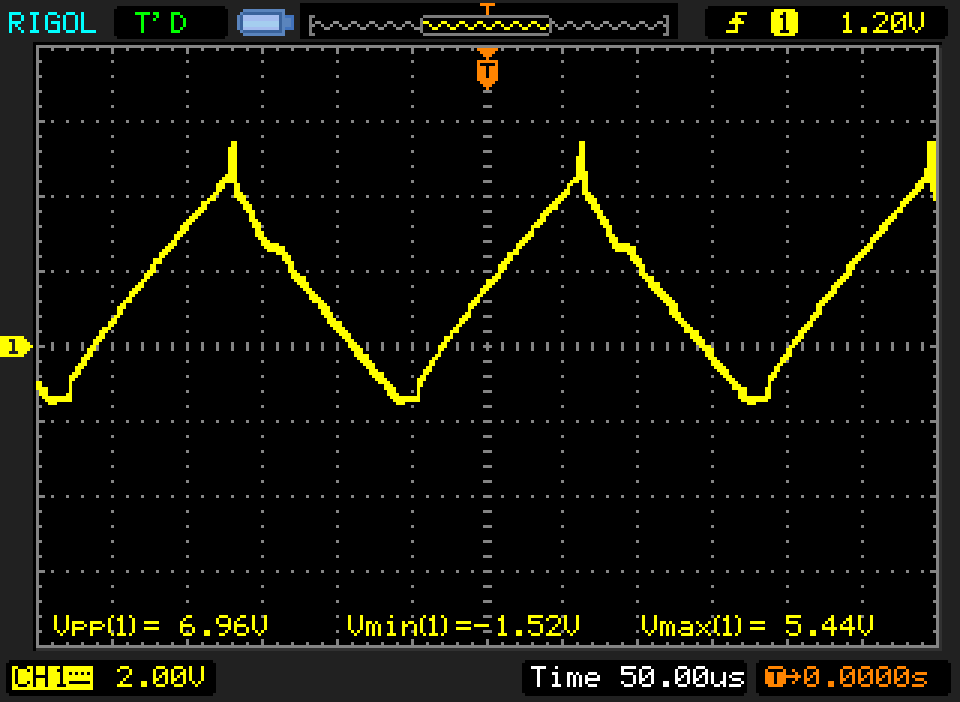
\includegraphics[width=\linewidth]{figuras/osc_3.png}
\caption{Señal 2 (\SI{2}{\volt\per div}, \SI{50}{\micro\second\per div}).}
\end{subfigure}\\[4pt]
\begin{subfigure}[b]{0.32\textwidth}
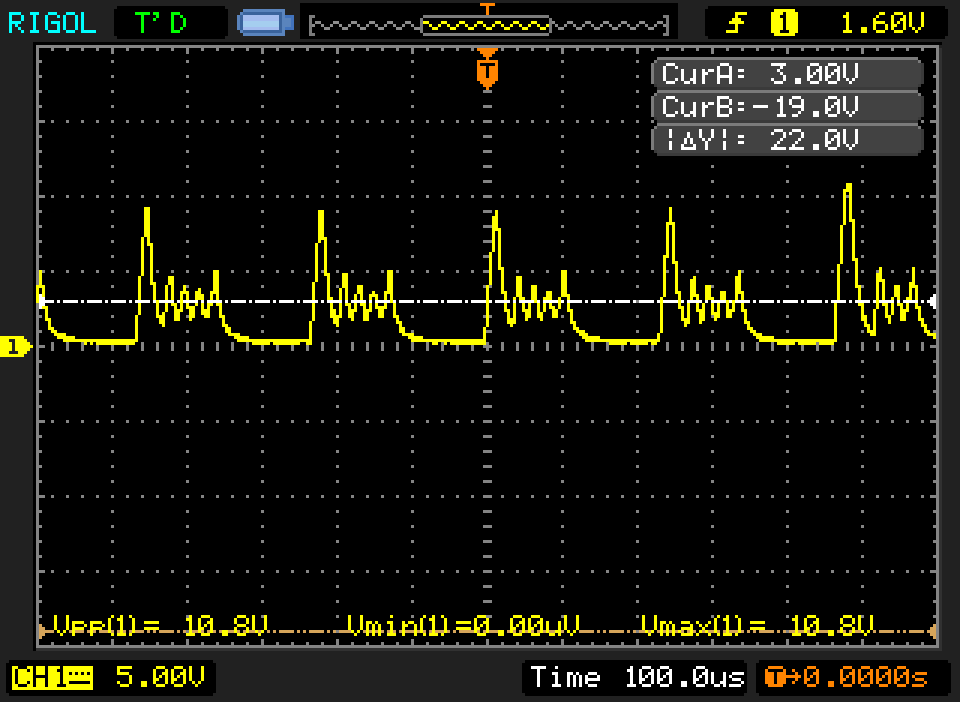
\includegraphics[width=\linewidth]{figuras/osc_4.png}
\caption{Señal 4 (\SI{5}{\volt\per div}, \SI{100}{\micro\second\per div}).}
\end{subfigure}\hfill
\begin{subfigure}[b]{0.32\textwidth}
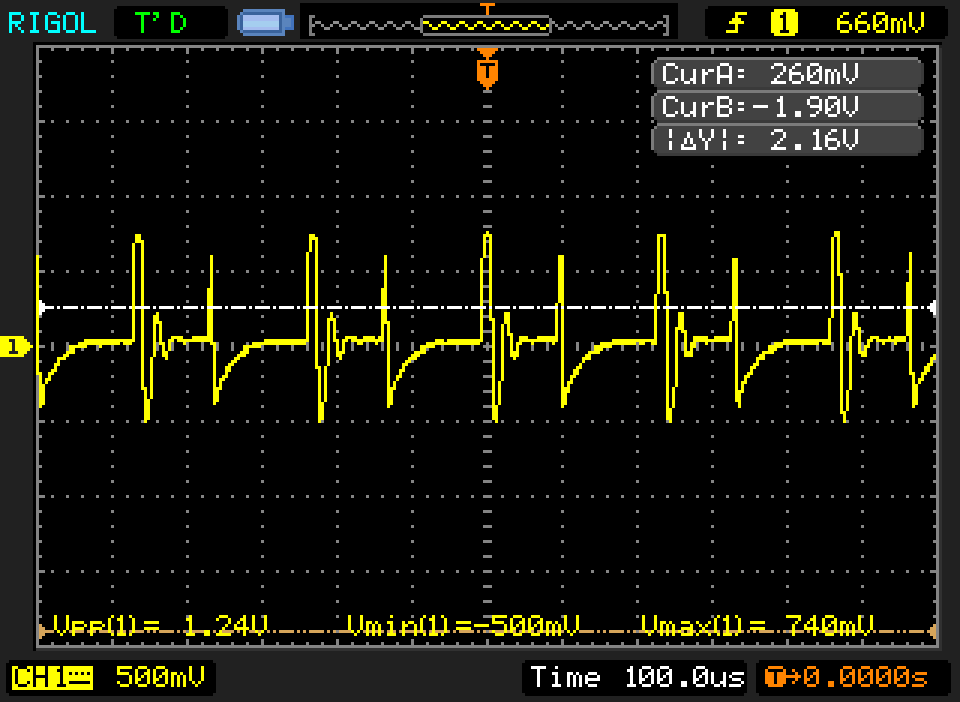
\includegraphics[width=\linewidth]{figuras/osc_5.png}
\caption{Impulsos $v_p$ (\SI{0,5}{\volt\per div}, \SI{100}{\micro\second\per div}).}
\end{subfigure}\hfill
\begin{subfigure}[b]{0.32\textwidth}
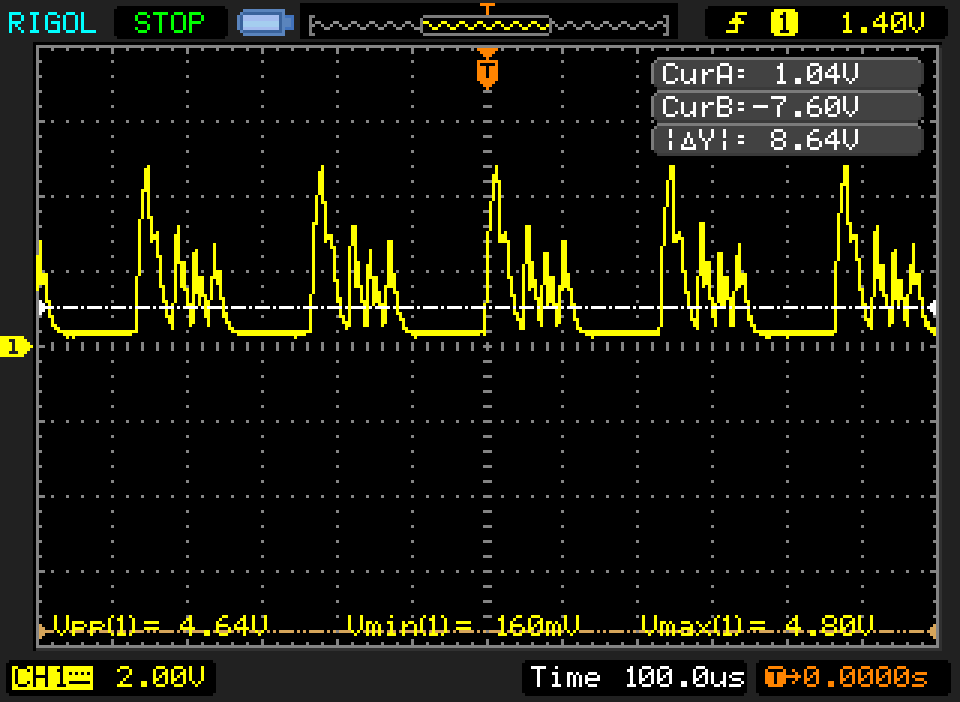
\includegraphics[width=\linewidth]{figuras/osc_6.png}
\caption{Señal 4 (\SI{2}{\volt\per div}, \SI{100}{\micro\second\per div}).}
\end{subfigure}
\caption{Capturas del osciloscopio. El marcador ``1'' del borde izquierdo indica el cero del canal en todas las capturas.}
\label{fig:capturas}
\end{figure*}

\subsection{Resultados: entrada, señal 1 y señal 2}
\label{sec:resultados}
La entrada (captura 1) es una cuadrada de \valu{2}{\medInBajo}{\volt} a \valu{2}{\medInAlto}{\volt} y \valu{3}{\medFrec/1000}{\kilo\hertz} según la medición automática del osciloscopio, con el nivel alto durante un \valu{0}{\medCiclo}{\percent} del período. La amplitud es un \valu{0}{100*(2.5-(\medInAlto-\medInBajo))/2.5}{\percent} menor que la nominal y la frecuencia, un \valu{1}{100*(4300-\medFrec)/4300}{\percent} menor.

La señal 1 (captura 2) tiene mesetas en \valu{2}{\medSUnoBajo}{\volt} y \valu{2}{\medSUnoAlto}{\volt}. Su excursión, \valu{2}{\medSUnoAlto-\medSUnoBajo}{\volt}, es la de la entrada: la ganancia del restador es 1, como se diseñó. La señal 2 (captura 3) es una triangular con rampas rectas, que sube mientras la señal 1 está en alto. Para no confundir sus vértices con los picos que aparecen sobre ellos, se calcularon intersecando rectas ajustadas a las rampas: \valu{2}{\medSDosVertMin}{\volt} y \valu{2}{\medSDosVertMax}{\volt}, con pendientes de \valu{1}{1000*\medSDosPendSub}{\volt\per\milli\second} y \valu{1}{1000*\medSDosPendBaj}{\volt\per\milli\second}.

Para comparar con la simulación sin mezclar los errores de ajuste con los de diseño, se repitió la simulación del circuito completo con la entrada medida (\valu{2}{\medInBajo}{\volt} a \valu{2}{\medInAlto}{\volt}, \valu{0}{\medFrec}{\hertz}) y con $P_2$ en la posición que reproduce el nivel medido de la señal 1. La Fig.~\ref{fig:medsim} superpone el resultado con las capturas 2 y 3, y la Tabla~\ref{tab:medicion} resume la comparación. La señal 1 simulada coincide con la medida en las dos mesetas, y la triangular medida tiene la forma, la fase y la linealidad de la simulada. Sus diferencias de amplitud y de nivel se analizan en la Sección~\ref{sec:problemas}.

\begin{figure}[!htb]
\centering
\begin{tikzpicture}
\begin{groupplot}[
    group style={group size=1 by 2, vertical sep=6pt, xticklabels at=edge bottom},
    tp2, height=3.8cm, xmin=0, xmax=600, xtick={0,100,...,600},
]
\nextgroupplot[ylabel={S1 [V]}, ymin=-1.4, ymax=2.5, ytick={-1,0,1,2}, legend pos=north east, legend columns=2]
\addplot[cmed, line width=1.6pt] table[x=t, y=v] {datos/med2.dat};
\addplot[cs1] table[x=t, y=s1] {datos/medida_sim.dat};
\legend{Medida, Simulada}
\nextgroupplot[ylabel={S2 [V]}, ymin=-2.4, ymax=6.4, ytick={-2,0,2,4,6}, xlabel={Tiempo [\si{\micro\second}]}]
\addplot[cmed, line width=1.6pt] table[x=t, y=v] {datos/med3.dat};
\addplot[cs2] table[x=t, y=s2] {datos/medida_sim.dat};
\end{groupplot}
\end{tikzpicture}
\caption{Capturas 2 y 3 digitalizadas, superpuestas con la simulación del circuito excitado con la entrada medida y con $P_2$ en la posición del ensayo.}
\label{fig:medsim}
\end{figure}

\begin{table}[!htb]
\centering
\caption{Comparación entre la medición y la simulación con la entrada medida.}
\label{tab:medicion}
\footnotesize
\setlength{\tabcolsep}{3pt}
\begin{tabular}{@{}llccc@{}}
\toprule
\textbf{Señal} & \textbf{Magnitud} & \textbf{Consigna} & \textbf{Simulada} & \textbf{Medida} \\
\midrule
Entrada & Bajo / alto [\si{\volt}] & 0 / 2,5 & \multicolumn{2}{c}{\val{2}{\medInBajo} / \val{2}{\medInAlto}} \\
 & Frecuencia [\si{\hertz}] & 4300 & \multicolumn{2}{c}{\val{0}{\medFrec}} \\
\midrule
S1 & Bajo / alto [\si{\volt}] & $-1$ / 1,5 & \val{2}{\simMedSunoBajo} / \val{2}{\simMedSunoAlto} & \val{2}{\medSUnoBajo} / \val{2}{\medSUnoAlto} \\
\midrule
\multirow{4}{*}{S2} & Mín. / máx. [\si{\volt}] & $-1{,}5$ / 4 & \val{2}{\simMedSdosMin} / \val{2}{\simMedSdosMax} & \val{2}{\medSDosVertMin} / \val{2}{\medSDosVertMax} \\
 & Pico a pico [\si{\volt}] & 5,5 & \val{2}{\simMedSdosVpp} & \val{2}{\medSDosVertVpp} \\
 & Nivel medio [\si{\volt}] & 1,25 & \val{2}{\simMedSdosMed} & \val{2}{\medSDosVertCentro} \\
 & Pend. sub. / baj. [\si{\volt\per\milli\second}] & $\pm 47{,}3$ & $\pm$\val{1}{(\simMedSdosVpp)/(0.5e3/\medFrec)} & \val{1}{1000*\medSDosPendSub} / \val{1}{1000*\medSDosPendBaj} \\
\midrule
\multirow{2}{*}{S4} & Impulsos por período & 2 & 2 & 1 \\
 & Pico [\si{\volt}] & 1 & 1,00 & \val{1}{\medCSeisMax} y \val{1}{\medCCuatroMax} \\
\bottomrule
\end{tabular}
\end{table}
